\documentclass[]{article}
\usepackage{listings}
\usepackage{graphicx}
\usepackage{float}
 
\floatstyle{ruled}
\newfloat{program}{thp}{lop}
\floatname{program}{Snippet}


\begin{document}

\title{Visualizing Software Projects in JavaScript}
\author{Tim Disney}
\date{}

\maketitle

\lstset{showstringspaces=false}

\begin{abstract}
  Visualization techniques have been used to help programmers deepen their understanding of large software projects. However the existing visualization techniques have focused on static languages where type information can be determined at compile-time. This paper describes a new visualization tool aimed at the dynamic language JavaScript.
\end{abstract}

\section{Introduction}
\label{sec:introduction}
Software is hard. Programmers spend much of their time managing the increasing complexities of software projects. One way to alleviate some portion of the difficulty in building and understanding a software project has been the use of visualization techniques. There have been a number of tools created to help visualize the structure and relationships between packages and classes \cite{solidsx, haskellvis} and dependencies \cite{idea, stan4j}. Unfortunately these tools only work for static languages where the types in the system can be determined at compile-time. To the best of the author's knowledge there are no visualization tools for dynamic languages which create and mutate their types are runtime.

This paper presents a visualization tool for JavaScript, a dynamic language used primarily in web browsers. This tool visualizes the structure of objects in a JavaScript application by using a node and link style graph. Changes to the object structure of the program are captured during run-time and represented visually by morphing the graph.

This paper is structured as follows: section \ref{sec:background} gives an overview of JavaScript, section \ref{sec:method} describes how the visualization is created, section \ref{sec:results} describes the author's experiences using the tool, section \ref{sec:related} gives an overview of related work, section \ref{sec:future} describes possible future work and section \ref{sec:conclusion} concludes.

\section{Background}
\label{sec:background}
JavaScript \cite{ECMA-262} is a dynamic language primarily used in client-side web applications. Once regarded as a toy scripting language its popularity has increased in recent years due to its use in complex web applications such as Gmail and Google Maps.

JavaScript provides support for object oriented techniques but uses a prototype-based object system as opposed to the more traditional class-based system found in languages such as Java or C++. Objects in JavaScript are collections of mutable key/value properties roughly analogous to maps in Java or dictionaries in Python. The potential objects an application uses are not defined before instantiation, instead objects are instantiated and then mutated into their necessary form as the application executes.

When object are created at the top level of a script (i.e. not inside functions as local variables) they are added as properties to a global object called {\tt window} in the browser setting. For example after the code in snippet \ref{snip:code} is executed the {\tt window} object will contain three properties: {\tt myObj} which is an object with {\tt foo} and {\tt baz}, {\tt myFun} which is a function, and {\tt globalVariable} which is the number 22.

\begin{program}[here]
\begin{verbatim}
var myObj = {
  foo: "bar",
  baz: 42.34
};

function myFun(){
  var localVariable = 5;
  globalVariable = 22;
}
\end{verbatim}
\caption{Example JavaScript code}
\label{snip:code}
\end{program}


\section{Method}
\label{sec:method}
Basically two things are happening. First there is some JavaScript that runs to collect all the data that matters. It runs by grabbing the {\tt window} global object and doing a depth-first search through each of the objects. As it walks each node (object) in the graph is constructs a separate object that will be used in the visualization tool. Essentially we are simplifying the object data that exists in the global object so that it can be more easily translated into the visualization.

There is some interesting filtering of the data going on. By default each browser provides a number of functions at the global level which are often not very interesting to the developer. By default these are ignored. The collector also does not walk down DOM elements. These are the elements that represent the elements displayed in the browser window. Since the focus is on the application and not the display these are currently being ignored. It also ignores objects that have been seen before to prevent creating circular references. This could be seen as a problem since it is sometimes very useful to know that an object is referenced by multiple names. For example the jQuery library has two alias that can be used ({\tt \$} and {\tt jQuery}) and there is good reason to visualize this relation. Only the first name discovered by the collector is currently being displayed but this could and probably should be changed in the future.

Array are another interesting special case in the collector. Since arrays are often used to hold large amounts of data (e.g. 1000s of elements) the collector will do some truncation of arrays if they exceeded a set maximum number of elements (currently set at 30).

Once the simplified object has been created it is passed to a visualization tool called the JavaScript InfoVis Toolkit (JIT) \cite{jit}. JIT then transforms the json object into a visualization in the browser. It uses canvas to draw the vis inside the browser window. There are some controls on the browser window to give some options to the user. Coloring of the graph can be turned on or off, the size of the canvas can be changed, maximum depth to draw, and which object to start with.


\section{Results}
\label{sec:results}
During development I actually managed to discover a programming flaw in the underlying JIT visualization library I was using. It appears that the programmers of JIT forgot to use the {\tt var} keyword when assigning to a variable called {\tt that}. I noticed this while testing out the change morphing, the {\tt that} variable showed up making me think that there was an error in my code but it was obvious from the visualization that the values being stored in {\tt that} had to do with the internals of JIT.

Use of a variable called {\tt that} is actually a standard pattern in JavaScript development. It is usually used to store a particular value of the {\tt this} object in a closure. Because the {\tt var} keyword was not used the assignment to {\tt that} was placed into the global object. This is a potential source of bugs since multiple closures could possible be in conflict about the contents of {\tt that}.


One of the goals of this visualization was to see the difference between a ``messy'' project and a ``clean'' project. Though the definitions are a bit fuzzy the intuition behind the terms is that a ``messy'' project has lots of objects in the global namespace while a ``clean'' project has relatively few. The reason for the value judgement in the terms is that when many things are in the same namespace the chance for unintentional conflict is greater and since JavaScript's type system is so dynamic the point of failure is later sometimes resulting in subtle runtime bugs. Also with a ``clean'' project structure understandibility and learning is facilatated. It is easier to find things when they have been grouped into hierarchies.

\begin{figure}[h]
  \begin{center}
    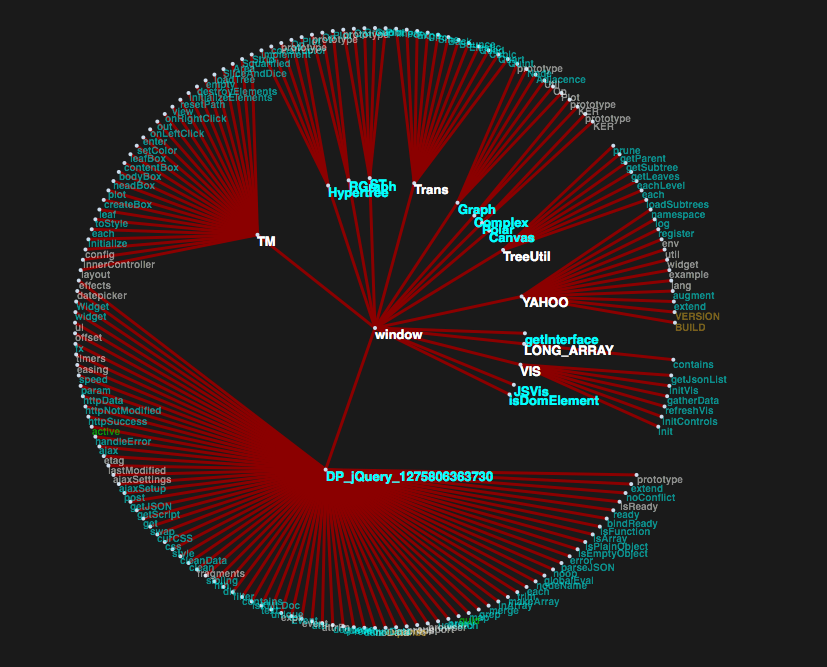
\includegraphics[scale=.25]{clean.png}
  \end{center}
  \caption{Clean Project}
  \label{fig:clean}
\end{figure}

To see if the visualization would work well for visualzing the difference between a ``messy'' and ``clean'' project I ran JSVis on two different projects. One was a project I had worked on several years ago when I was first learning how to program in JavaScript. The other was the use of the calenadar widget for YUI. Admittedly the comparison is in someways unfair since the functionality of the two projects is very different however since the underlying structure is so different it does works as an illustrative example. As can be seen in fig \ref{fig:clean} there are around half a dozen items in the top level with many more items under each of them. In contrast figure \ref{fig:messy} has tons of items in the top level making it very difficult to make out one from the other.


\begin{figure}[h]
  \begin{center}
    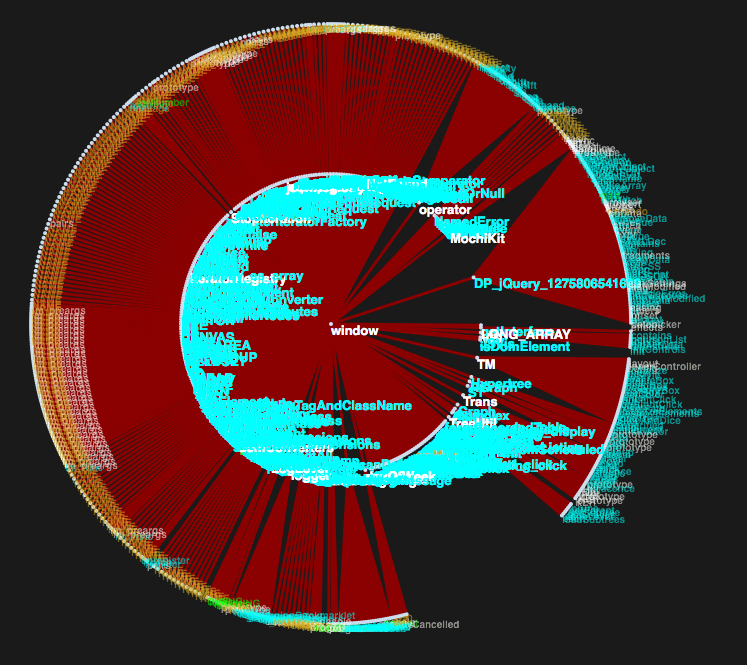
\includegraphics[scale=.25]{messy.png}
  \end{center}
  \caption{Messy Project}
  \label{fig:messy}
\end{figure}

\begin{figure}[h]
  \begin{center}
    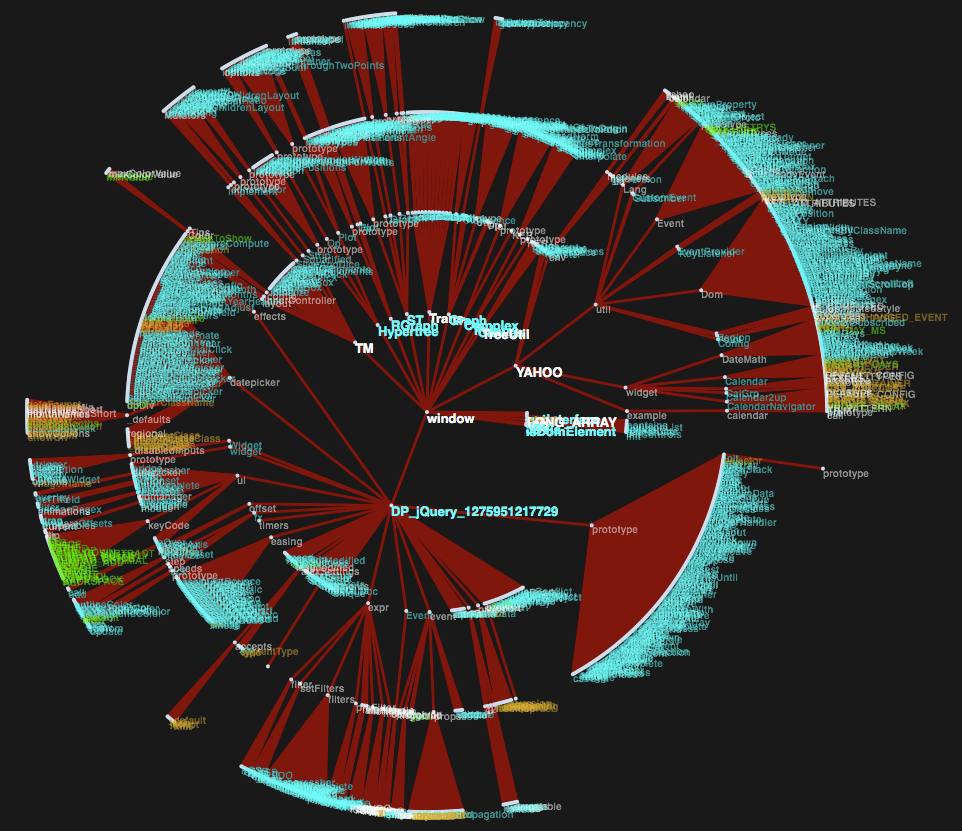
\includegraphics[scale=.2]{deep-window.png}
  \end{center}
  \caption{Global object four levels deep}
  \label{fig:deep-window}
\end{figure}

\begin{figure}[h]
  \begin{center}
    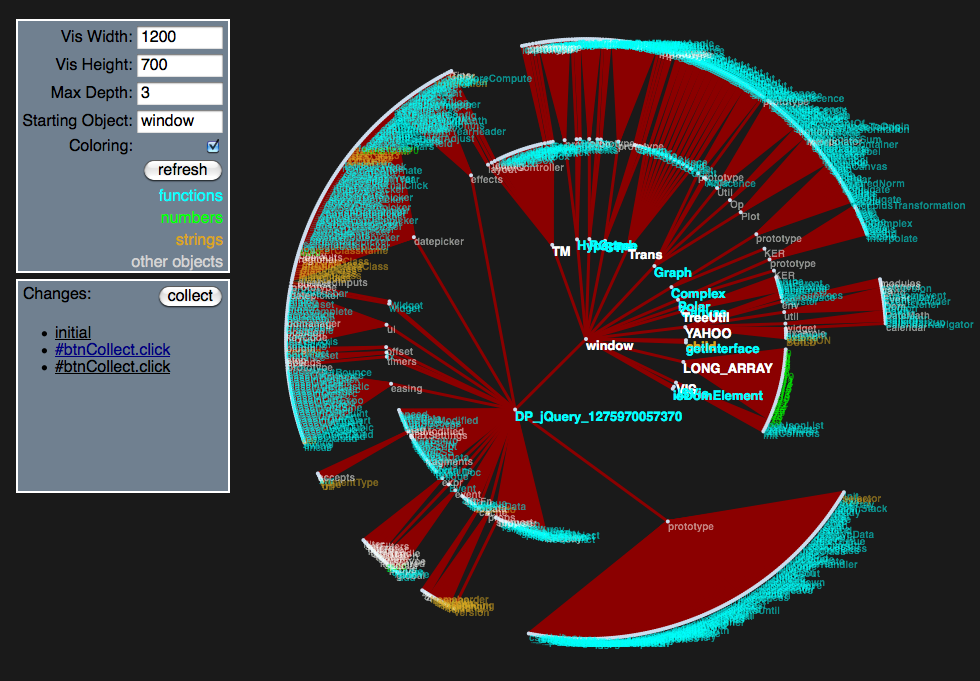
\includegraphics[scale=.2]{interface.png}
  \end{center}
  \caption{Global object three levels deep with interface}
  \label{fig:interface}
\end{figure}

\begin{figure}[h]
  \begin{center}
    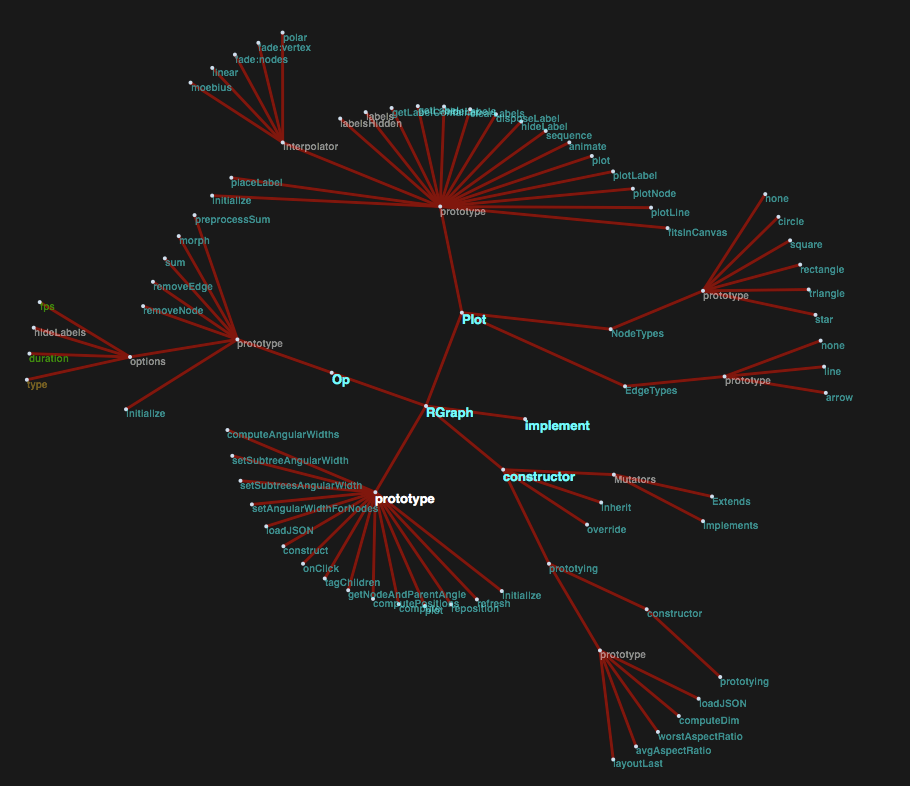
\includegraphics[scale=.2]{rgraph.png}
  \end{center}
  \caption{RGraph object four levels deep}
  \label{fig:rgraph}
\end{figure}

\begin{figure}[h]
  \begin{center}
    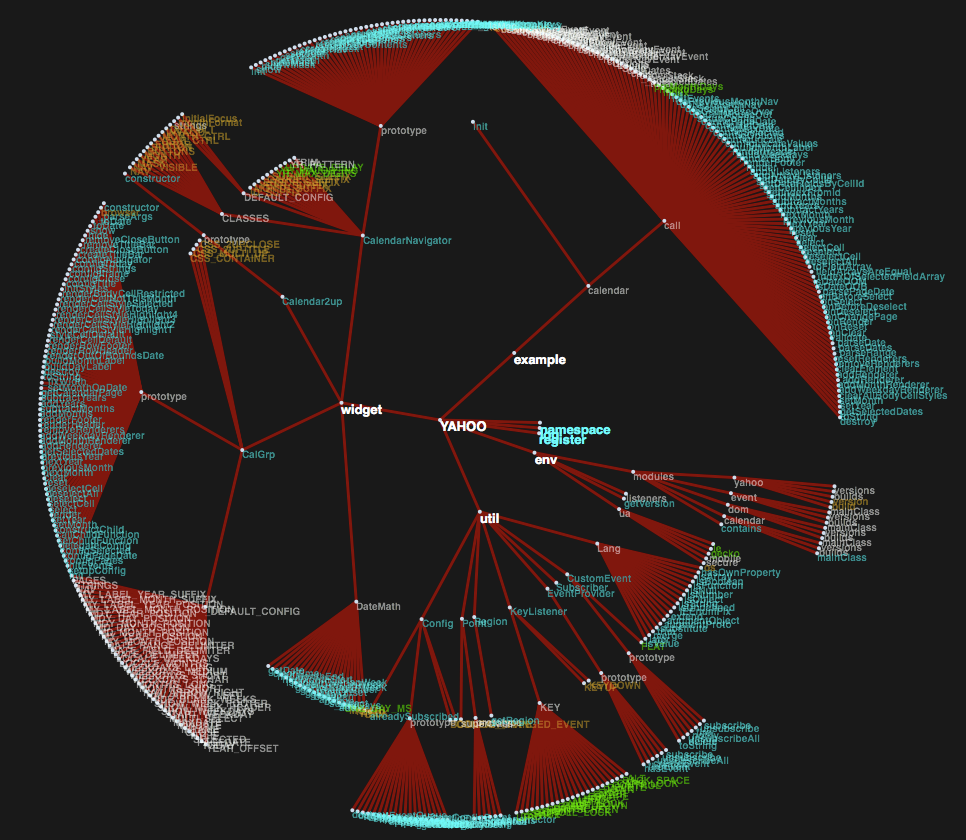
\includegraphics[scale=.2]{yahoo.png}
  \end{center}
  \caption{YAHOO object four levels deep}
  \label{fig:yahoo}
\end{figure}

\section{Related Work}
\label{sec:related}
That which has gone before.

\section{Future Work}
\label{sec:future}
What could be done.
%TODO: talk about collecting more object data from JS engines

\section{Conclusion}
\label{sec:conclusion}
What did we do again?

\bibliographystyle{plain}
\bibliography{report}

\end{document}



